\documentclass[11pt]{article}
\usepackage{amsmath, bm}
\usepackage{ntheorem}
\usepackage{fullpage}
\usepackage{amsfonts}
\usepackage{setspace}
\usepackage{graphicx}
\usepackage{ctex}
%\usepackage{titlesec} 

%\newcommand{\mycmd}[2]{$\mathbb{#1}^{#2}$} falied to perform

%\theorembodyfont{\normalfont}
%\newtheorem*{definition*}{Definition}
%
\theorembodyfont{\normalfont}
\newtheorem{remark}{Remark}
%
%\theorembodyfont{\normalfont}
%\newtheorem*{errata*}{Errata}
%
\theorembodyfont{\normalfont}
\newtheorem{question}{Question}

\newcommand{\divergence}{\nabla\cdot}
\newcommand{\bmv}{\bm{v}}
%
%\theorembodyfont{\normalfont}
%\newtheorem{theorem}{Theorem}
%
%\theorembodyfont{\normalfont}
%\newtheorem*{proposition*}{Proposition}
%
%\newcommand{\ind}[1][17]{\setlength{\parindent}{#1pt}} % Create an indentation of length 17pt

%\usepackage{mathrsfs} % 6 maths fonts

%\titlespacing{\section}{0pt}{20pt}{20pt}
\title{笔试答卷}
\author{侯怡枫}
%\date{}
%\doublespacing
\onehalfspacing
\newcounter{mycount}




\begin{document}



\maketitle

答卷中用到的源代码都将在Email附件中附上。所有程序都在Linux Ubuntu LTS 16.04操作系统上编译。

\section*{第1题}

首先用R将数据plot出来获得一个直观的感受。
\begin{figure}[h]
	\centering
	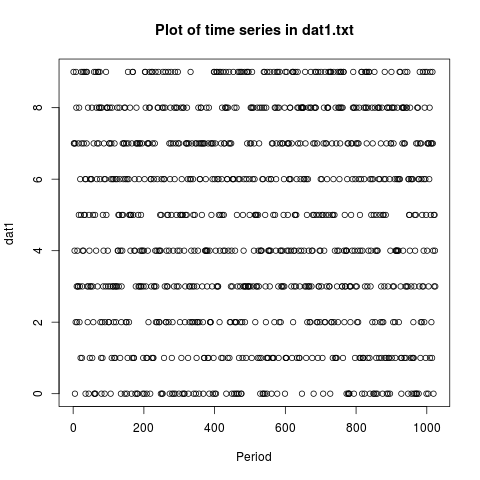
\includegraphics[scale=0.4]{dat1_plot.png}
	\caption{dat1.txt 中数据的时间序列图}
\label{dat1_plot}
\end{figure}

根据图\ref{dat1_plot}, 改时间序列并不呈现确定性时间趋势(deterministic time trend)。然后,图\ref{dat1_acf} 展示改题数据的样本ACF。
\begin{figure}[h]
	\centering
	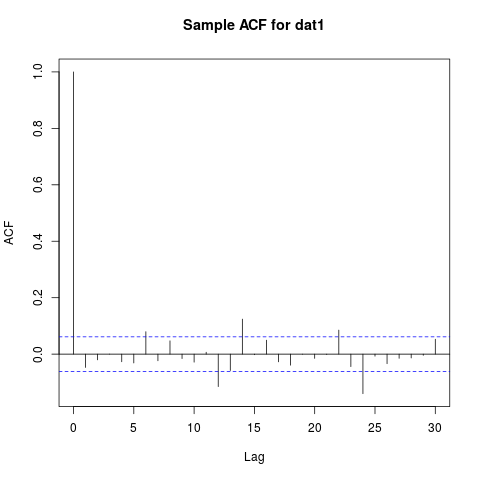
\includegraphics[scale=0.4]{dat1_acf.png}
	\caption{dat1.txt 中数据的样本ACF plot}
\label{dat1_acf}
\end{figure}

从图\ref{dat1_acf}中可以看到,该序列和$k=1$的滞后项的样本相关系数接近1。这是存在单位根(有随机时间趋势)的很强的经验证据。所以答题者选择“存在单位根”作为原假设。

答题者计划使用ADF(augmented Dickey-Fuller)检验。为使用ADF检验,首先要选择一个信息标准(Information Criterion)来确定自回归的滞后步长(lag)。这里答题者选择AIC进行模型选择。对本题时间序列运行AIC后确定的滞后步长是24。

在确定步长后,




\bibliographystyle{plain}
\bibliography{Tornado}

\end{document}